\documentclass[12pt]{article}
\usepackage{cite}
\usepackage{graphicx}
\usepackage{geometry}
\usepackage{float}
\usepackage{multicol}
\usepackage{subfigure}

\geometry{left=2.0cm,right=2.0cm,top=2.5cm,bottom=2.5cm}

\title{
    \textbf{\Huge ECE385} \\
    \huge Fall 2020 \\
    \huge Experiment 9 \\[120pt]
    \textbf{\Huge SOC With Advanced Encryption Standard in SystemVerilog} \\[120pt]
    }

\author{
    \large Name: Zhou Qinren \\ 
            \quad\qquad Zhang Yichi \\
    \large Lab Section: LA3 \\
    \large TA's Name: Yu Yuqi
    }

\date{Dec. $8^{th}$ 2020}

\begin{document}
\setlength{\parindent}{0pt}
\maketitle
\newpage

\section{Introduction}
In this experiment, we implemented a 128-bit advanced encryption standard using software as an intellectual property core. We also implemented a corresponding decryption module. The AES encryptor receives a plain sequence and encrypts it and stores the encrypted information in some registers. The decryptor fetches the encrypted code in the registers and then decrypts it. 

\section{Written Description and Diagrams of the AES encryptor/decryptor}
\subsection{Software Encryptor}
The NIOS receives the plain information via console, and then encrypts it and store the encrypted information into some specific registers. The C code consists of some encryption help functions and a main function. The user enters a plain message using console, then the C code will store the message into an array of unsigned char. Then the user inputs the key, which will also be stored into an array. After that, the C code will generate the key expansion of the input key, and then perform the encryption. The process includes AddRoundKey, SubBytes, ShiftRows and MixColumns. AddRoundKEy takes the current message and a set of key as input, and performs an XOR operation. SubBytes substitute the current information with the information in a look-up table. ShiftRows shifts each row in the updating state by some offsets. MixColumns transforms the state via a separate invertible linear field. After the message is encrypted, the C code will store the encrypted message into some specific registers addressed by the pointer AES\_PTR.

\subsection{Hardware Decryptor}
The hardware consists of a register file and a controller. The register file is used to store the key, encrypted message, decrypted message, and control signals. The controller takes charge of the decryption process. The controller is essentially an FSM, and when the control signal Run is high, the controller starts the decryption, and go through many states. In our design, the FSM includes 7 states: Stop, KesExpansion, AddRoundKey, InvShiftRows, InvSubBytes, InvMixColumns and End. Each state does exactly what its name suggests, and some states also checks some other condition, so as to follow the right flow. 

\subsection{Hardware/Software Interface}
The avalon\_aes\_interface module is the interface that connects the software and hardware. It contains a register file of 16 32-bit registers. 0-3 stores the key, 4-7 stores the encrypted message, 8-11 stores the decrypted message, 14 stores the Start signal, and 15 stores the Done signal. NIOS sends data to the hardware using a pointer AES\_PTR. The pointer points to the base address of the hardware. When sending data, we have to specify the relative address of the registers, e.g., AES\_PTR[2] = something. For the hardware to send data to NIOS, it works similarly, e.g., some variable = AES\_PTR[2]. 
\begin{figure}[H]
    \centering
    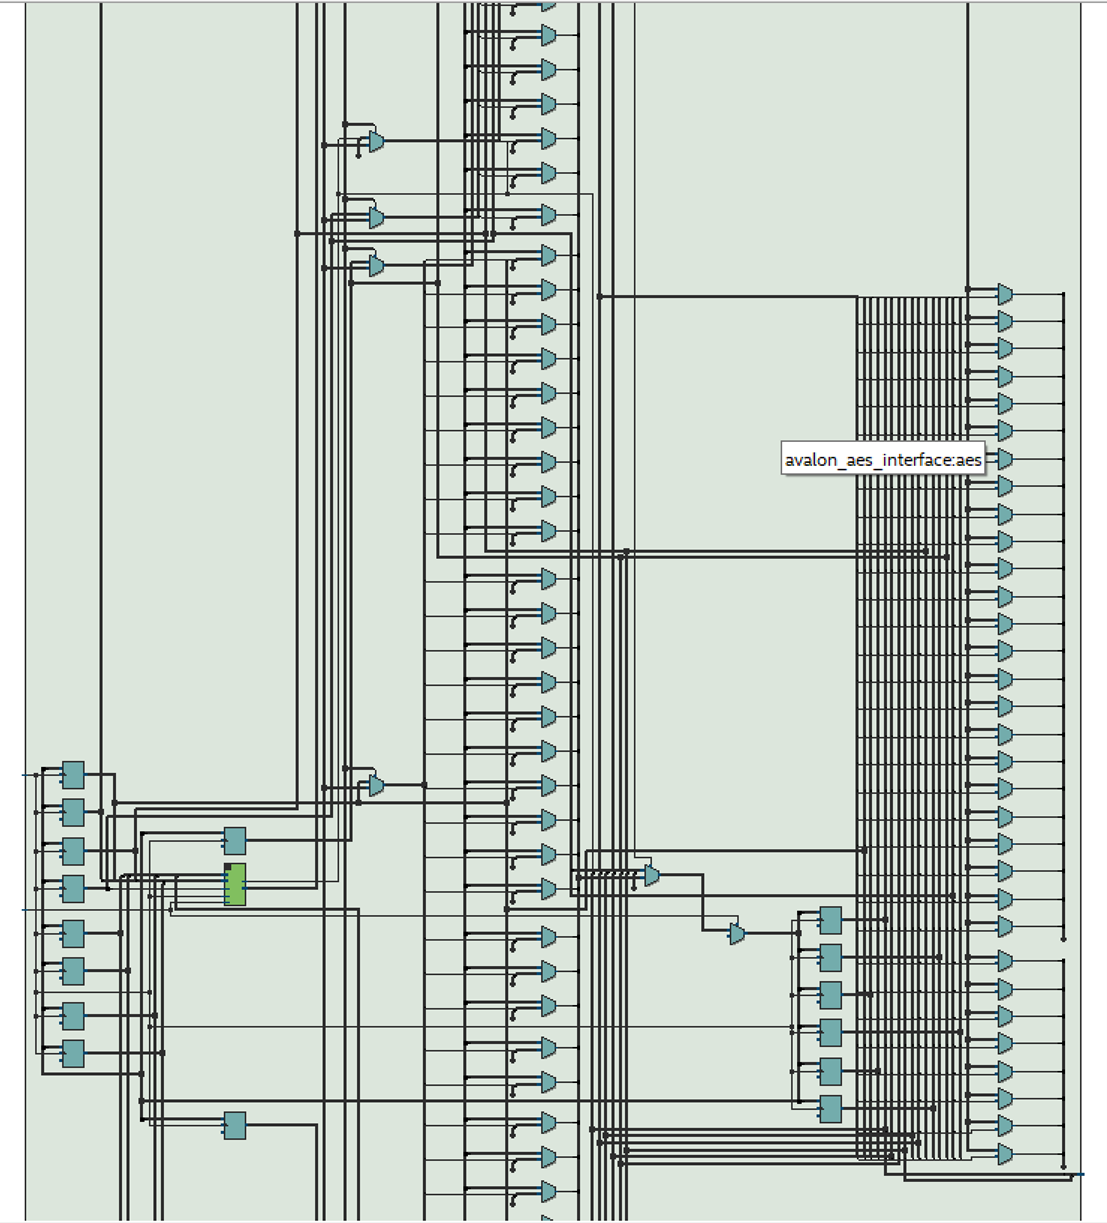
\includegraphics[width=15cm]{interface.png}
    \caption{RTL view of avalon\_aes\_interface.}
\end{figure}
The original graph is too large, we only captured the most complex part of it. The rest part is similar but simpler.

\subsection{Block Diagram}
\begin{figure}[H]
    \centering
    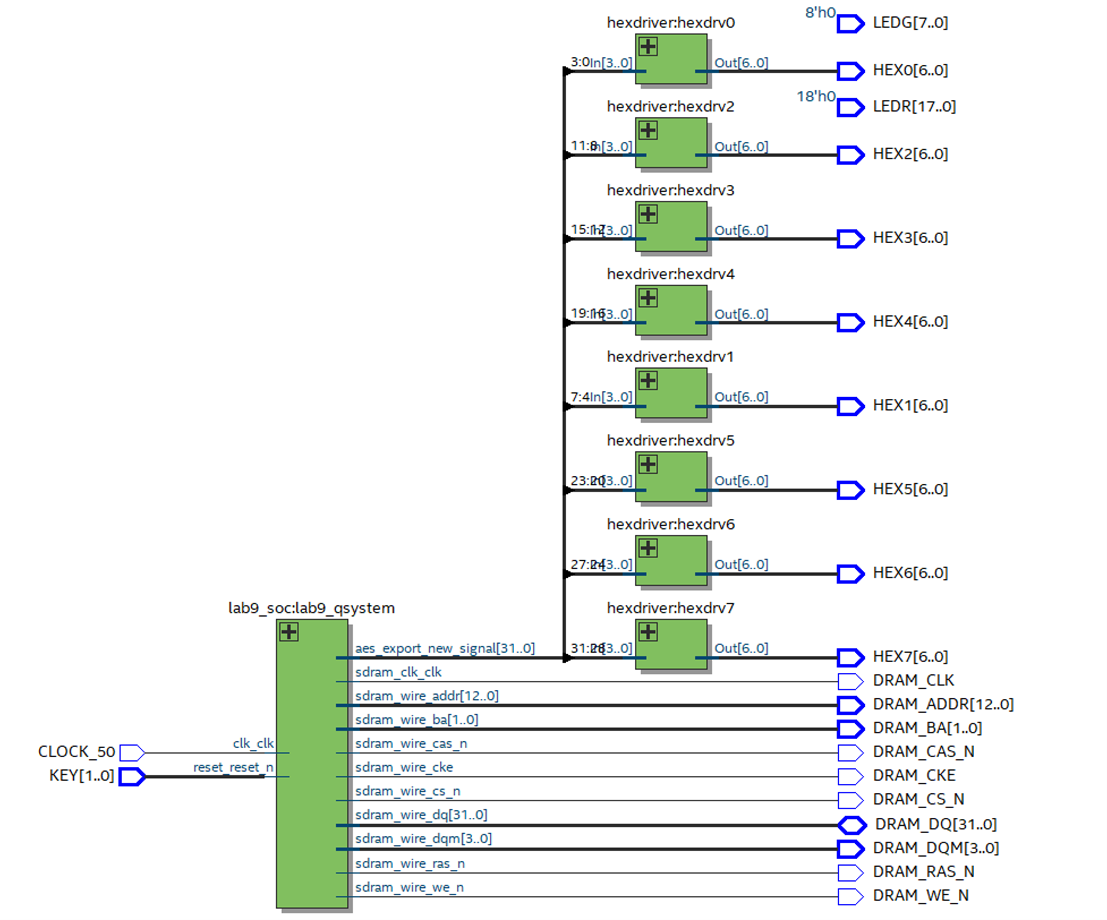
\includegraphics[width=15cm]{blockdiagram.png}
    \caption{Top level block diagram.}
\end{figure}

\subsection{State Diagram of AES Decryptor Controller}
The first FSM is the outer state machine, it takes Start and Reset as input signals. If Start is high, then it goes to Execute state and triggers the inner FSM to start. When the decryption completes, the FSM goes to Done state, and outputs the Done signal.
\begin{figure}[H]
    \centering
    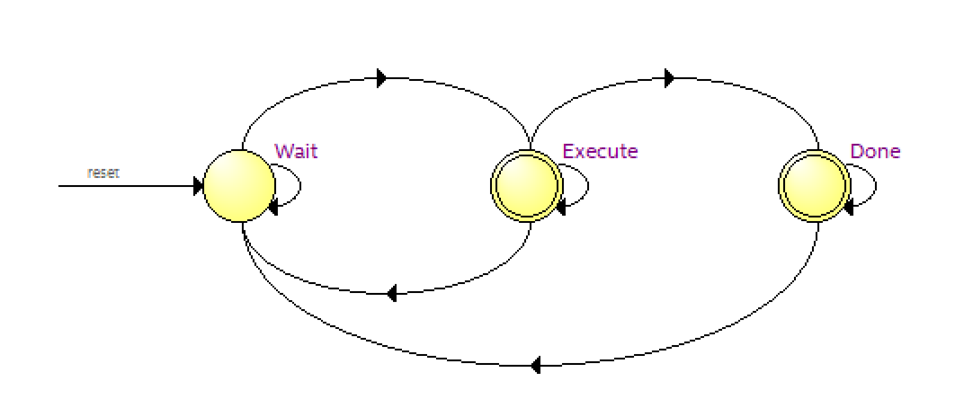
\includegraphics[width=12cm]{FSM_outer.png}
    \caption{Outer FSM.}
\end{figure}

The inner FSM is the whole process of decryption. It stays in Stop state until the outer FSM triggers. Then it goes to many states to go through the decryption state. 
\begin{figure}[H]
    \centering
    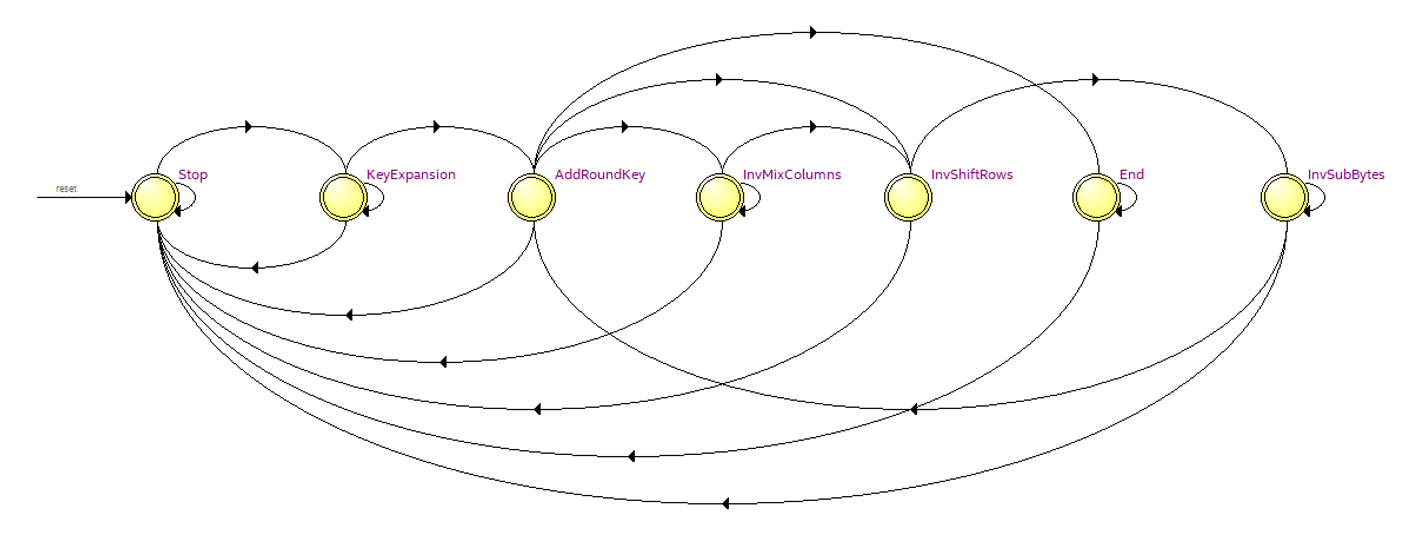
\includegraphics[width=18cm]{FSM_inner.png}
    \caption{Inner FSM.}
\end{figure}

\section{Module Description}
\textbf{Module}: KeyExpansionOne \\ 
\textbf{Inputs}: clk, [127:0] oldkey, [7:0] Rcon \\ 
\textbf{Outputs}: [127:0] newkey \\
\textbf{Description}: It calls SubBytes and search the LUT Rcon to calculate a 128-bit key. \\ 
\textbf{Purpose}: It takes in an old key and outputs a new key for next AddRoundKey. \\

\textbf{Module}: KeyExpansion \\ 
\textbf{Inputs}: clk, [127:0] Cipherkey \\ 
\textbf{Outputs}: [1407:0] KeySchedule \\
\textbf{Description}: It constantly calls KeyExpansionOne. \\ 
\textbf{Purpose}: It calculates all 11 keys needed and combines and outputs them as a 1407 bits KeySchedule. \\

\textbf{Module}: SubBytes \\ 
\textbf{Inputs}: clk, [7:0] in \\ 
\textbf{Outputs}: [7:0] out \\
\textbf{Description}: This is a $16 \times 16$ LUT. \\ 
\textbf{Purpose}: It helps us to convert a 8-bit input to a specific byte for encryption. \\

\textbf{Module}: InvSubBytes \\ 
\textbf{Inputs}: clk, [7:0] in \\ 
\textbf{Outputs}: [7:0] out \\
\textbf{Description}: This is a $16 \times 16$ LUT. \\ 
\textbf{Purpose}: It helps us to convert a 8-bit input to a specific byte for decryption. \\

\textbf{Module}: InvSubState \\ 
\textbf{Inputs}: clk, [127:0] in \\ 
\textbf{Outputs}: [127:0] out \\
\textbf{Description}: It constantly calls InvSubBytes. \\ 
\textbf{Purpose}: It helps us to convert a 128-bit input to specific 16 bytes for decryption. \\

\textbf{Module}: InvShiftRows \\ 
\textbf{Inputs}: [127:0] data\_in \\ 
\textbf{Outputs}: [127:0] data\_out \\
\textbf{Description}: Consider and store the 128-bit input as a $4 \times 4$ matrix, each element is 2 bytes. This module keeps the first row unchanged, circular right shift the second row once, circular right shift the third row twice and circular right shift the fourth row three times. \\ 
\textbf{Purpose}: This is a step in decryption. \\

\textbf{Module}: InvMixColumns \\ 
\textbf{Inputs}: [31:0] in \\ 
\textbf{Outputs}: [31:0] out \\
\textbf{Description}: Search the GF\_MUL LUT to convert a 32-bit input to 4 specific bytes. \\ 
\textbf{Purpose}: It does inverse mix columns for one column. \\

\textbf{Module}: AddRoundKey \\ 
\textbf{Inputs}: [127:0] in, [1407:0] keys, [3:0] round \\ 
\textbf{Outputs}: [127:0] out \\
\textbf{Description}: It calculates the output of AddRoundKey according to the round the FSM is in. \\ 
\textbf{Purpose}: This is a step in decryption. \\

\textbf{Module}: counter \\ 
\textbf{Inputs}: CLK, RESET, in \\ 
\textbf{Outputs}: [3:0] out \\
\textbf{Description}: A counter. Every time the in signal is high, we add 1 to the counter. \\ 
\textbf{Purpose}: This can be the counter counting 10 rounds for KeyExpansion and counting 9 rounds of InvShiftRows, InvSubBytes, AddRoundKey and InvMixColumns. \\

\textbf{Module}: AES \\ 
\textbf{Inputs}: CLK, RESET, AES\_START, [127:0] AES\_KEY, [127:0] AES\_MSG\_ENC \\ 
\textbf{Outputs}: AES\_DONE, [127:0] AES\_MSG\_DEC \\
\textbf{Description}: An FSM. \\ 
\textbf{Purpose}: This is the FSM for decryption. It takes in the encrypted message, calls the helper modules and outputs the decrypted message. \\

\textbf{Module}: avalon\_aes\_interface \\ 
\textbf{Inputs}: CLK, RESET, AVL\_READ, AVL\_WRITE, AVL\_CS, [3:0] AVL\_BYTE\_EN, [3:0] AVL\_ADDR, [31:0] AVL\_WRITEDATA \\ 
\textbf{Outputs}: [31:0] AVL\_READDATA \\
\textbf{Description}: It calls the AES module to do the decryption and stores the result to the SDRAM. Also, it writes the data into the SDRAM or reads the data out of the SDRAM based on the avalon signals. \\ 
\textbf{Purpose}: This is the interface that connects the software and hardware. The hardware writes data into SDRAM through this module and the software writes data into or reads data out of SDRAM through this module. \\

\textbf{Module}: lab9\_top \\ 
\textbf{Inputs}: CLOCK\_50, [1:0] KEY \\ 
\textbf{Outputs}: [7:0] LEDG, [17:0] LEDR, [6:0] HEX0, [6:0] HEX1, [6:0] HEX2, [6:0] HEX3, [6:0] HEX4, [6:0] HEX5, [6:0] HEX6, [6:0] HEX7, [12:0] DRAM\_ADDR, [1:0] DRAM\_BA, DRAM\_CAS\_N, DRAM\_CKE, DRAM\_CS\_N, [3:0] DRAM\_DQM, DRAM\_RAS\_N, DRAM\_WE\_N, DRAM\_CLK \\
\textbf{Inouts}: [31:0] DRAM\_DQ \\
\textbf{Description}: It connects the signal of all the hardwares. \\ 
\textbf{Purpose}: This is the top level module for lab9. \\

\begin{figure}[H]
    \centering
    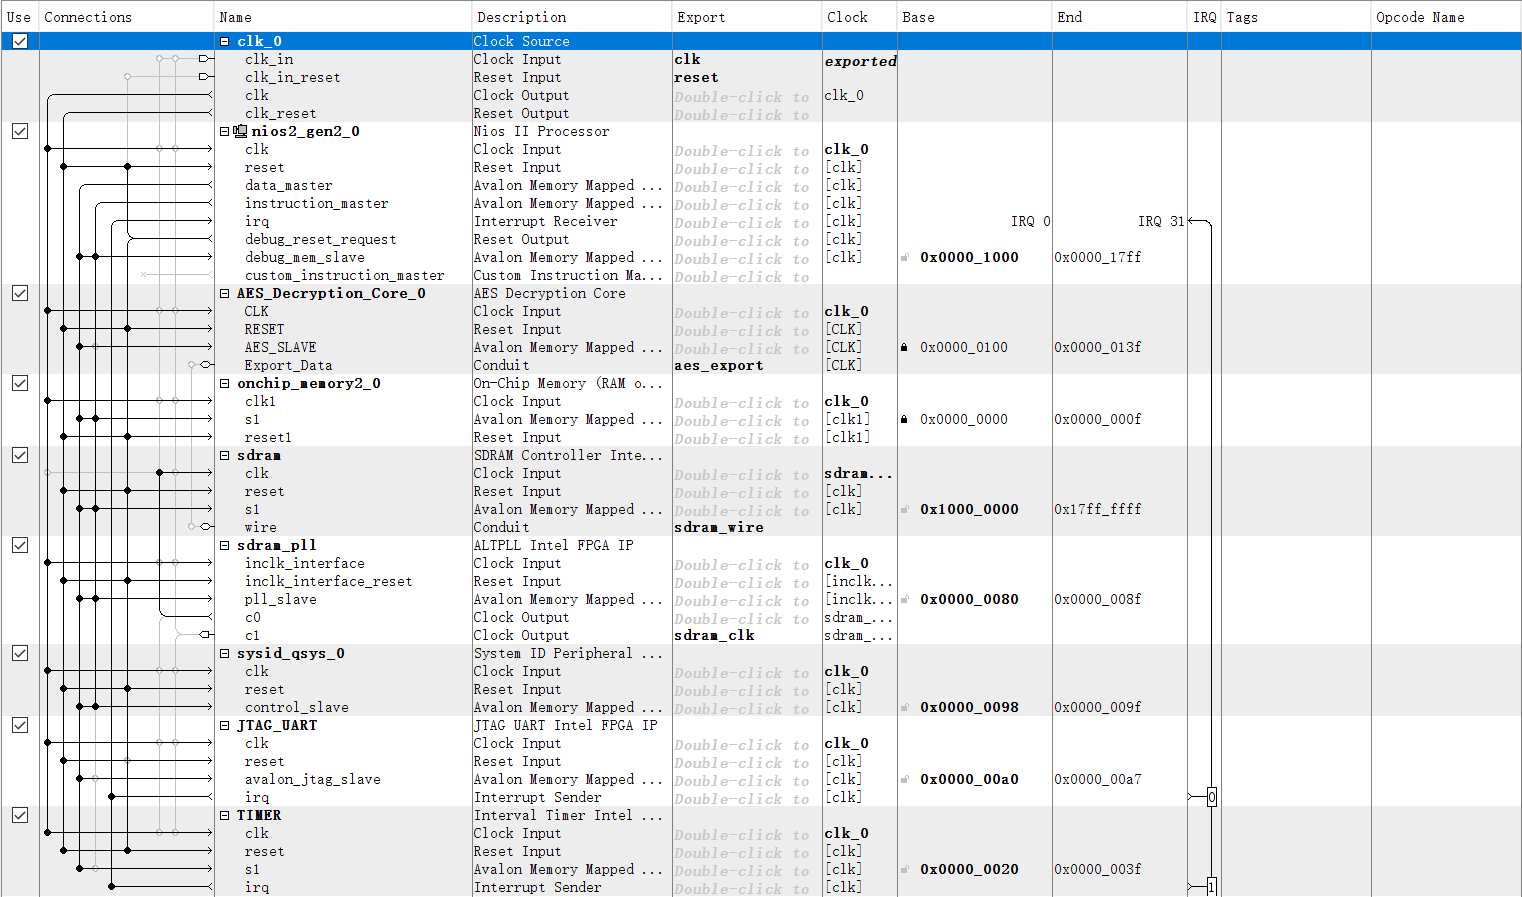
\includegraphics[width=18cm]{platform.png}
    \caption{Platform designer view.}
\end{figure}

This is the hardware platform for our lab9 design. We build this platform by deleting the otg\_hpi modules and keycode module and adding AES\_Decryption\_core\_0 and TIMER modules on the basis of the platform of lab8. 

\begin{figure}[H]
    \centering
    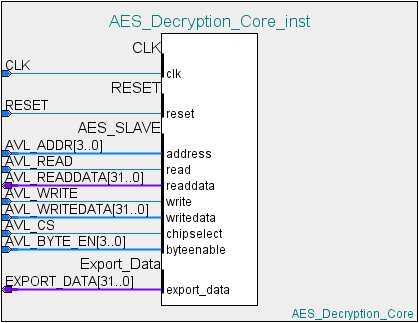
\includegraphics[width=10cm]{AES_decryption_core.png}
    \caption{AES\_Decryption\_core\_0 instance.}
\end{figure}

AES\_Decryption\_core\_0 is an IP we made based on the avalon\_aes\_interface module. It is controlled by the NIOS-II through signals in Avalon-MM bus. 

\begin{figure}[H]
    \centering
    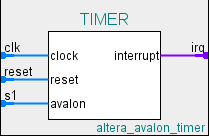
\includegraphics[width=8cm]{timer.png}
    \caption{Timer instance.}
\end{figure}

TIMER module is used to measure the encryption and decryption time by sending periodic interrupts.

\section{Annotated Simulation of the AES Decryptor}
\begin{figure}[H]
    \centering
    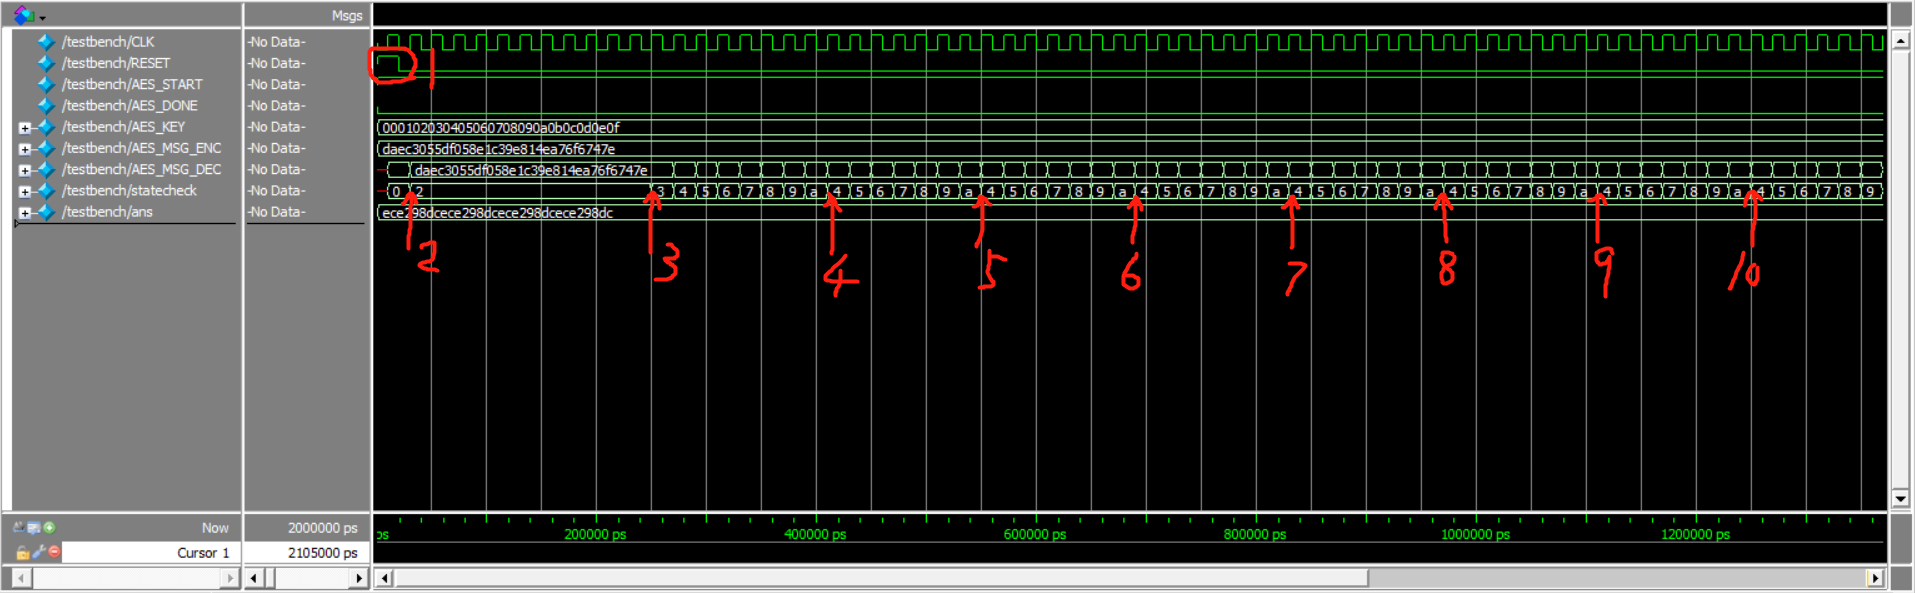
\includegraphics[width=18cm]{simulation1.png}
    \caption{Annotated simulation1.}
\end{figure}
\begin{figure}[H]
    \centering
    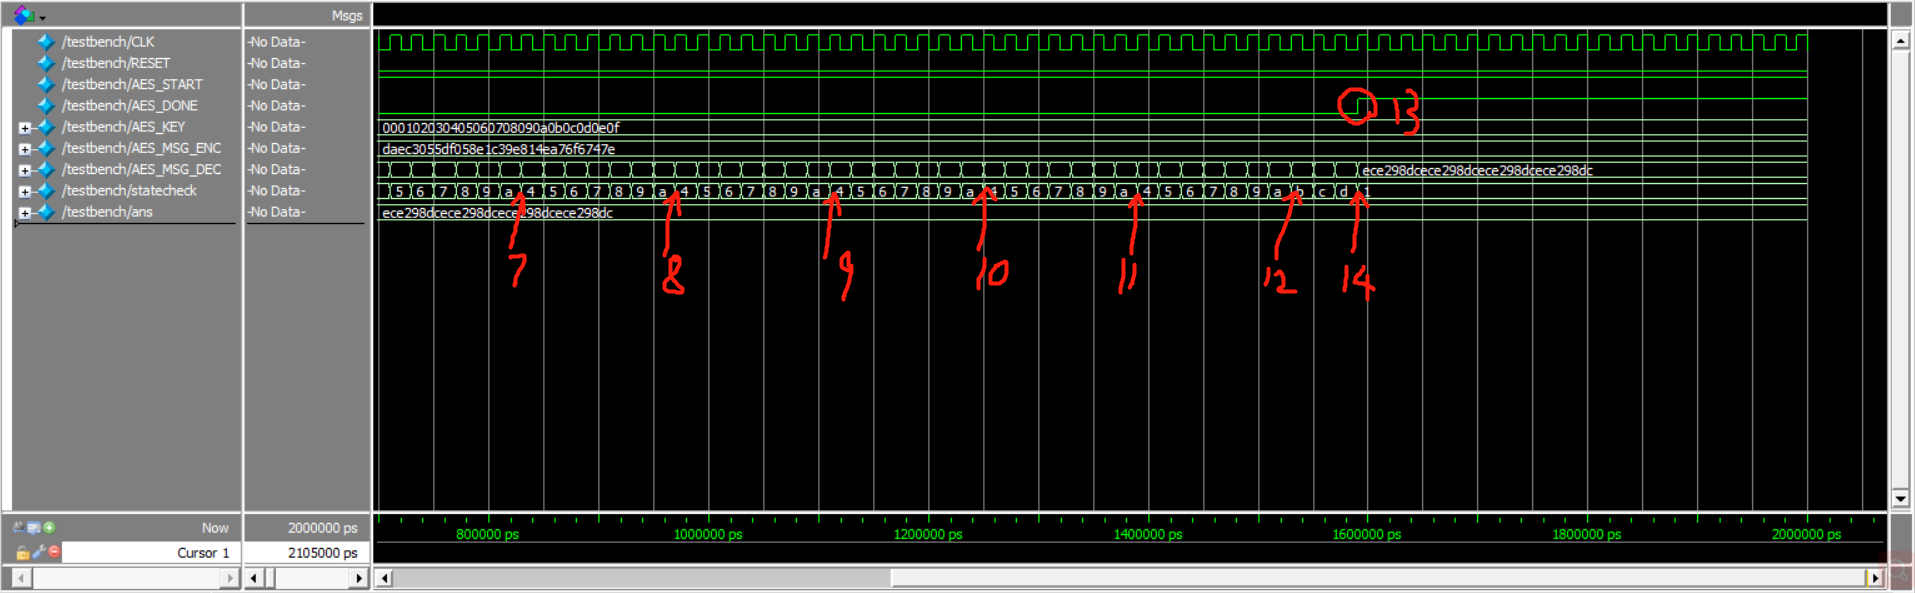
\includegraphics[width=18cm]{simulation2.png}
    \caption{Annotated simulation2.}
\end{figure}
state 0: Halt\\
state 1: Done\\
state 2: KeyEx\\
state 3: firstAddRoundKey\\
state 4: nineInvShiftRows\\
state 5: nineInvSubBytes\\
state 6: nineAddRoundKey\\
state 7: InvMixColumns\_1\\
state 8: InvMixColumns\_2\\
state 9: InvMixColumns\_3\\
state a: InvMixColumns\_4\\
state b: lastInvShiftRows\\
state c: lastInvSubBytes\\
state d: lastAddRoundKey\\

The reset signal is set high at mark 1 for one cycle. Right after this cycle, at mark 2, the FSM enters the KeyExpansion state for 10 cycles where the module KeyExpansion calculate and store the keyschedule for later use. At mark 3, the FSM finishes KeyExpansion and starts to decrypt. After the firstAddRoundKey and nine rounds of InvShiftRows, InvSubBytes, AddRoundKey and InvMixColumns (from mark 3 to mark 12), the FSM then does the last InvShiftRows, InvSubBytes and AddRoundKey.
Finally, at mark 13 and 14, the FSM enters the Done state where it holds the decrypted values and set the AES\_DONE signal high. As we can see, the final result is the same as the ans signal where stores the real answer of decryption.

\section{Post Lab Questions}
\begin{table}[H]
    \centering
    \resizebox*{7cm}{5cm}{
        \begin{tabular}{|l|l|l|l|}
        \hline
        LUT           & 5979            \\ \hline
        DSP           & 0               \\ \hline
        BRAM          & 571392          \\ \hline
        Flip-Flop     & 2877            \\ \hline
        Frequency     & 119.9MHz        \\ \hline
        Static Power  & 102.54mW        \\ \hline
        Dynamic Power & 72.82mW         \\ \hline
        Total Power   & 243.48mW        \\ \hline
        \end{tabular}
    }
    \caption{Design statistics table for the multiplier.}
\end{table}

Question: Which would you expect to be faster to complete encryption/decryption, the software or hardware? Is this what your results show? (List your encryption and decryption benchmark here) \\

Answer: We expect the hardware to be faster. Yes, the result approves that. We can see that the hardware is approximately 800 times faster. \\
\begin{figure}[H]
    \centering
    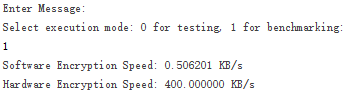
\includegraphics[width=12cm]{benchmark.png}
    \caption{Benchmark.}
\end{figure}

Question: If you wanted to speed up the hardware, what would you do? (Note: restrictions of this lab do not apply to answer this question) \\

Answer: Build a complete LUT for InvMixColumns. Now we compute InvMixColumns column by column. If there is a complete LUT that takes in a 128-bit input, search the LUT and directly outputs the result, it will be much faster. \\

\section{Conclusion}
\subsection{Functionality}
In this lab, we first achieved encryption in software then decryption in hardware. When we built the FSM for decryption we made a mistake that we reset the state where we temporarily stored the result of decryption to be the encrypted message instead of 128-bit zeros. Later we found that when the reset is triggered the encrypted message had not been loaded. It was just some random numbers. We have to store the encrypted message to the state after the reset process. Finally, all the functions work well.

\subsection{About the Lab Manual}
It would be much nicer if the requirements are highlighted.

\newpage
\bibliography{}
\bibliographystyle{ieeetr}
\end{document}